\providecommand{\VarRectoVerso}{\oneside}
\documentclass[french,11pt]{article}

\usepackage[T1]{fontenc}
\usepackage[utf8]{inputenc}
\usepackage{babel}
\usepackage{fullpage}
\usepackage{lmodern}
\usepackage{graphicx}
\usepackage{enumerate}
\usepackage{xspace}
\usepackage{amsmath}
\usepackage{amsfonts}
%\usepackage{mathenv}
\usepackage{amsthm}

\newtheorem{remarque}{Remarque}[subsubsection]
\newtheorem{definition}{Définition}[subsubsection]
\newtheorem{proposition}{Proposition}[subsubsection]
\newtheorem{theoreme}{Théorème}[subsubsection]
\newtheorem{exemple}{Exemple}[subsubsection]

%\usepackage{verbatim}
%\usepackage{moreverb} %pour utiliser plus de fonctions de verbatim

\newcommand{\chapterEt}[1]{\chapter*{#1}\addcontentsline{toc}{chapter}{#1}}
\newcommand{\sectionEt}[1]{\section*{#1}\addcontentsline{toc}{section}{#1}}

\newcommand{\R}{\mathbb{R}}
\newcommand{\x}{\bar{x}}



\title{Complexité}
\author{Danielle Quichaud}
\usepackage{amsmath}
\usepackage{graphicx}
\begin{document}
\maketitle
\tableofcontents
\section{TD1}

\begin{exercice}{Fibonacci}

\[ \begin{cases} u_n = u_{n-1} + u_{n-2} \\ u_1 = 1 \\ u_0= 0 \end{cases} \]

\textit{Équation caractéristique} 
\[x^2-x-1 = 0\]
\[ \Delta = 1+4=5 >0 \]
\[ \textit{2 racines distincts } \frac{1 \pm \sqrt{5}}{2} \]
\[ u_n = a \left(\frac{1 - \sqrt{5}}{2}\right)^n + b \left(\frac{1 + \sqrt{5}}{2}\right)^n \]

\textit{Calcul de a et b} 
\[ u_0 = 0 = a +b \]
\[ u_1 = 1 = a \left(\frac{1 - \sqrt{5}}{2}\right) + b \left(\frac{1 + \sqrt{5}}{2}\right) \]
\[ \Rightarrow \]
\[ a + b = 0 \Leftrightarrow b = -a \]
\[ \sqrt(5) (b-a) = 2 \]
\[ \Leftrightarrow \]
\[ b = \frac{1}{\sqrt{5}} \]
\[ a = -\frac{1}{\sqrt{5}} \]

\[ u_n = \frac{1}{\sqrt{5}} \left[ \left( \frac{1 + \sqrt{5}}{2} \right)^n - \left( \frac{1 - \sqrt{5}}{2} \right)^n \right] \]


\end{exercice}

\begin{exercice}
\[ \begin{cases} u_n = 4 u_{n-1} - 4 u_{n-2} + 2 n \\ u_1 = 1 \\ u_0 = 0 \end{cases} \]

On a bien $f(n)$ de la forme $b^n P(n)$ avec $b = 1$ et $P(n) = 2n$, $d^o P = 1$.

\textit{Équation caractéristique} 
\[ (x^2-4x+4)(x-1)^2 = 0 \]
\[ \Ra (x-2)^2(x-1)^2 = 0 \]
\[ \Ra \textit{ 2 et 1 racines doubles} \]
\[ \Ra u_n=(an+b)2^n+(cn+d) \]
\[ \textit{(sol gen + sol part)} \]

\textit{Calcul de c et d} en écrivant que $u_n=cn+d$ est une solution particulière de $t$.
\[ cn+d=4[c(n-1)+d]-4[c(n-2)+d]+2n \] 
\[ cn+d+4c-4d-8c+4d=2n \]
\[ cn+d-4c=2n \]
\[ \Ra \begin{cases} c=2 \\ d-4c=0 \Ra d=8 \end{cases} \]
\[ \Ra u_n=(an+b)2^n+2n+8 \]

\textit{Calcul de a et b}
\[ \begin{cases} u_0=0=b+8 \Ra b=-8 \\u_1=1=2(a+b)+10 \Ra 2a=7 \Ra a=\frac{7}{2} \end{cases} \]

\[ \Ra u_n=(\frac{7}{2}n-2)2^n+2n+8 \]

\end{exercice}

\begin{exercice}
\[ \begin{cases} u_n=u_{n-1}+u_{n-3}-u_{n-4} \textit{ pour } n\ge 4 \\ u_n=n \textit{ pour } 0 \le n \le 5 \end{cases} \]

\textit{Équation caractéristique} 
\[ x^4-x^3-x+1=0 \]
\[ \textit{solution évidente : } 1 \]
\[ (x-1)(x^3-1)=0 \]
\[ (x-1)(x-1)(x^2+x+1)=0 \]
\[ (x-1)^2(x^2+x+1)=0 \]
\[ x^2+x+1 \textit{ n'a pas de solution réelles } \]
\[ 2 \textit{ racines complexes } \frac{-1 \pm 
i \sqrt{3}}{2} = \pm e^{i\frac{2\pi}{3}} \]
\[ \textit{ce sont les racines cubiques de l'unité : } j \textit{ et } j^2 \]

\[ u_n=(an+b)+cj^n+dj^{2n} \]

Calcul de a, b, c et d à partir des conditions initiales
\[ \begin{disarray}{r c l}
\begin{cases}u_0=0=b+c+d \\ 
u_1=1=a+b+cj+dj^2 \\
u_2=2=2a+b+cj^2+dj \\
u_3=3=3a+b+c+d \end{cases}
\Ra\begin{cases} a=1 \\ 
b+c+d=0 \\
b+cj+dj^2=0 \\
b+cj^2+dj=0 \end{cases}

&\Ra& \begin{cases} a=1 \\ 
b=-c-d \\
c(j-1)+d(j^2-1)=0 \\
c(j^2-1)+d(j-1)=0 \end{cases}\\

&\Ra& \begin{cases} a=1 \\ 
b=c=d=0 \end{cases}
\end{disarray} \]
 
\end{exercice}
 
\begin{exercice}

\[ \begin{cases} u_n=3u_{n-1}^2 \textit{ pour } n \ge 1 \\ u_0=1 \end{cases} \]

Il faut se ramener à une équation de récurrence linéaire qu'on résoud par la méthode des l'équation caractéristique. On passe donc par les logarithmes.

\[ \log u_n =n\log 3+2\log u_{n-1} \]

On change de varible : $v_n=\log u_n$.
\[ \begin{cases} v_n=2v_{n-1}+n\log 3 \\
v_0=\log u_0=0 \end{cases} \]

Le second membre est bien de la forme $b^nP(n)$ avec $b=1$ et $P(n)=n\log 3$ ($d^o P=1$), on utilise donc la méthode de l'équation caractéristique.

\[ (x-2)(x-2)^2=0 \]
\[ v_n=a2^n+bn+c \]

Calcul de b et de c
\[ bn+c=2[b(n-1)+c]+n\log 3 \]
\[ -bn-c-2b=n\log 3\]
\[ \begin{cases} b=-\log 3 \\ c+2b=0 \Ra c=-2b=2\log 3 \end{cases} \]

Calcul de a à partir de $v_0$
\[ v_0=0=a+c \Ra a=-2\log 3 \]
\[ v_n=-2^{n+1}\log 3-n\log 3+2\log3 \]
\[ v_n=[-2^{n+1}-n+2]\log 3 \]
\[ \Ra u_n=e^{v_n}=e^{[-2^{n+1}-n+2]\log 3} \]
\[ u_n=3^{-2^{n+1}-n+2} \]

\end{exercice}

\begin{exercice}

\[ \begin{cases} T(n)=aT(\frac{n}{n})+g(n) \\ T(1)=1 \end{cases} \]

On obtient ce genre d'équations avec des algos du type diviser pour régner. Problème décomposé en sous problèmes de taille $\frac{n}{b}$. $g(n)$ est le cout de la décomposition, et de la recomposition.

Hypothèse : $n$ puissance de $b$ : $n=b$
\[ \begin{cases} T(b^k)=aT(b^{k-1})+g(b^k) \\ T(b^0)=1 \end{cases} \]

On fait ler changement de variable : $u_k=T(b^k)$
\[ \begin{cases}u_k=au_{k-1}+g(b^k) \\ u_0=1 \end{cases}\]

Par la méthode des facteurs sommants

\[ \begin{cases}
	u_k=au_{k-1}+g(b^k)\\
	u_{k-1}=au_{k-2}+g(b^{k-1})\\
	...\\
	u_k=au_1+g(b)
\end{cases}\]

\[u_k=a^ku_0+\sum_{i=0}^{k-1} a^ig(b^{k-1})\]

\[\Ra u_k=a^k+\sum_{i=0}^{k-1} a^ig(b^{k-1})\]
\end{exercice}

\section{TD2}
\subsection{Series génératrices pour résoudre des équations de récurrence}
\begin{exercice}
\[ \begin{cases}
	u_n = 5u_{n-1} - 6u_{n-2}$ pour n $\ge2\\
	u_0=0,u_1 = 1
\end{cases}\]

Faire apparaitre la génératrice $u(x) = \sum_{n\ge0} u_n x^n$\\

$\ra$ \underline{\textbf{Multiplier par :}} $x^n$\\
$u_nx^n = 5u_{n-1}x^n - 6u_{n-2}x^n$ pour $n \ge 2$\\

$\ra$ \textbf{\underline{Sommer ces équations pour faire apparaitre la série génératrice :}}\\
$\sum_{n\ge2}u_nx^n = 5u_{n-1}x^{n-1} - 6x^2 \sum_{n\ge2} u_{n-2}x^{n-2}$\\

%$u(x)-u_0-u_2x = 5x \sum_{n\ge2}u_{n-1}$\\
%... voir Cannibal : fait
\[ u(x) = \sum_{n>=2}^{} u_nx^n\]
On obtient après sommage
\[ \sum_{n>=2}^{} u_nx^n = 5\sum_{n>=2}^{} u_{n-1}x^{n-1} - 6\sum_{n>=2}^{} u_{n-2}x^{n-2}\]
\[ \begin{disarray}{r c l}u(x)-u_0-u_1x &=& 5x\sum_{n>=2}^{} u_{n-1}x^{n-1} - 6x^2\sum_{n>=2}^{} u_{n-2}x^{n-2}\\
&=& 5x\sum_{n>=1}^{} u_{n}x^{n} - 6x^2\sum_{n>=0}^{} u_{n}x^{n}\end{disarray}\]
\[ u(x)-u_0-u_1x = 5x[u(x)-u_0]-6x^2u(x)\]
$\ra$ avec $u_0 = 0, u_1 = 1$
\[\Ra u(x) - x = 5xu(x) - 6x^2u(x)\]
\[u(x)[6x^2-5x+1]=x\]
\[u(x)=\frac{x}{6x^2-5x+1}\]
$\ra$ racines de $6x^2-5x+1$
\[\delta = 25-24 = 1 >0 \ra 2\]

racines distinctes $\frac{5 \pm 1}{12}$ donne $\frac{1}{2}$ ou $\frac{1}{3}$

\[u(x)=\frac{x}{6(x-\frac{1}{2})(x-\frac{1}{3})}=\frac{a}{x-\frac{1}{2}}+\frac{b}{x-\frac{1}{3}}\]
%fini

$\ra X(x-\frac{1}{2})$ puis $x = \frac{1}{2}$ => $a=\frac{\frac{1}{2}}{6(\frac{1}{2}-\frac{1}{3})} =  \frac{1}{2})$\\

$\ra X(x-\frac{1}{3})$ puis $x = \frac{1}{3}$ => $b=\frac{\frac{1}{3}}{6(\frac{1}{3}-\frac{1}{2})} = \frac{1}{3})$\\

$u(x) = \frac{1}{2(x-\frac{1}{2})} - \frac{1}{3(x-\frac{1}{3})} = \frac{1}{2x-1}-\frac{1}{3x-1} = \frac{1}{1-3x} - \frac{1}{1-2x}$\\

$\Ra$ utiliser $\frac{1}{1-cz} = \sum_{n \ge 0}c^nz^n \Ra$
\[ \begin{cases}
	\frac{1}{1-3x} = \sum_{n\ge0}3^nx^n\\
	\frac{1}{1-2x} = \sum_{n\ge0}2^nx^n
\end{cases}\]

% Voir Thibaud 2 : fait
\[\Ra u(x) = \sum_{n>=0}^{} u_{n}x^{n}=\sum_{n>=0}^{} 3^{n}x^{n}-\sum_{n>=0}^{} 2^{n}x^{n}\]
\[\sum_{n>=0}^{} (3^{n}-2^{n})x^{n}\]
$\Ra u_{n} = 3^{n}-2^{n}$ pour $n>=0$

\end{exercice}

\begin{exercice}
Même travail sur le système suivant :
\[\begin{cases}
	u_n = 2u_{n-1} + u_{n-2} - 2u_{n-3} pour n>=3\\
	u_0 = 0, u_1 = u_2 = 1\\
\end{cases}\]

\[\sum_{n>=3}^{}u_nx^n = 2\sum_{n>=3}^{}u_{n-1}x^n + \sum_{n>=3}^{}u_{n-2}x^n - 2\sum_{n>=3}^{}u_{n-3}x^n\]
\[u(x)-u_0-u_{1}x-u_{2}x^2 = 2x\sum_{n>=2}^{}u_nx^n+x^2\sum_{n>=2}^{}u_nx^n-2x^3\sum_{n>=2}^{}u_nx^n\]


%fini
$u(x)-u_0 -u_1x - u_2x^2 = 2x [u(x)-u_0-u_2x] + x^2[u(x) - u_0] - 2x^3u(x)$\\
avec $u_0 = 0, u_1 = u_2 = 1$\\

$\Ra u(x) - x - x^2 = 2x u(x) - 2x^2 +x^2u(x) - 2x^3u(x)$\\

$u(x)[2x^3-x^2-2x+1] = x-x^2$\\

$\Ra u(x) = \frac{x(1-X)}{2x^3 - x^2 -2x +1}$\\

racines de $2x^3 -x^2 -2x +1$ :\\
Une racine évidente :\\
$2x^3 - x^2 - 2x + 1 = (x-1)(2x^2+x-1) \\= (x-1)(x+1)(2x-1)$ car -1 racine de $2x^2+x-1$\\



%Voir Thibaud 3 : Fait
\[\Ra u(x) = \frac{x(x-1)}{(x-1)(x+1)(2x-1)}=\frac{x}{(x+1)(2x-1)}=\frac{a}{1+x}+\frac{b}{1-2x}\]
$\ra x(1+x)$ puis $x=-1$ donne $a=\frac{-1}{1+2}=\frac{-1}{3}$

$x(1-2x)$ puis $x=\frac{1}{2}$ donne $b=\frac{\frac{1}{2}}{1+\frac{1}{2}}=\frac{1}{3}$
\[u(x) = \frac{1}{3}\left[\frac{1}{1-2x}-\frac{1}{1+x}\right]\]
utiliser 
\[\frac{1}{1-cz}=\sum_{n>=0}^{} c^{n}z^{n}\]
donne  \[\frac{1}{1-2x}=\sum_{n>=0}^{} 2^{n}x^{n}\]
et \[\frac{1}{1+x}=\sum_{n>=0}^{} (-1)^{n}x^{n}\]
\[u(x) = \frac{1}{3}\left[\sum_{n>=0}^{} 2^{n}x^{n}-\sum_{n>=0}^{} (-1)^{n}x^{n}\right]=\sum_{n>=0}^{} \frac{1}{3}\left[2^n-(-1)^n\right]x^n\]
\[\Ra u_n=\frac{1}{3}\left[2^n-(-1)^n\right]\]pour n $\ge$ 0
\end{exercice}
%fin
\begin{exercice}
\[ \begin{cases}
	u_n=3u_{n-1}-2u_{n-2} $ pour $ n\ge2\\
	u_0=u_1=0
\end{cases}\]

\[\sum_{n\ge2}u_nx^n = 3 \sum_{n\ge2}u_{n-1}x^n - 2\sum_{n\ge2}u_{n-2}x^n + 4\sum_{n\ge2}(n-2)x^n\]
Posons $u(x) =\sum_{n \ge 0} u_nx^n$\\
\[\dsr
u(x)-u_0-u_1x 
&=& 3x\sum_{n \ge 2}u_{n-1}x^{n-1} - 2x^2\sum_{n \ge 2}u_{n-2}x^{n-2}+ 4x^2\sum_{n \ge 2}(n-2)x^{n-2}\\
&=& 3x\sum_{n \ge 1}u_{n}x^n - 2x^2\sum_{n \ge 0}u_nx^n + 4x^2\sum_{n \ge 0}nx^n\\
&=& 3x[u(x)-u_0] -2x^2u(x)+4x^2\sum_{n \ge 0}nx^n\findsr\]
avec $u_0 = u_1 = 0 $ et $\displaystyle\sum_{n \ge 0}nx^n=\frac{x}{(1-x)^2}$\\

% voir Thibaud 4 : fait
\[u(x)=3xu(x)-2x^2u(x)+\frac{4x^3}{(1-x^2)^2}\]
\[\Ra u(x)[2x^2-3x+1]=\frac{4x^3}{(1-x^2)^2}\]
\[\Ra u(x)=\frac{4x^3}{(1-x^2)^2(2x^2-3x+1)}\]
or \[2x^2-3x+1 = (x-1)(2x-1)\]
\[u(x)=\frac{4x^3}{(1-x^2)^3(2x^2-3x+1)}=\frac{a}{1-2x}+\frac{b}{1-x}+\frac{c}{(1-2x)^2}+\frac{d}{(1-2x)^3}\]
$x(1-2x)$ puis $x=\frac{1}{2}$ donne $a=\frac{4(\frac{1}{2})^3}{(1-\frac{1}{2})^3}=4$

$x(1-x)^3$ puis $x=1$ donne $d=\frac{4}{1-2}=-4$

\[u(x)=\frac{4}{1-2x}-\frac{4}{(1-x)^3}+\frac{b}{1-x}+\frac{c}{(1-x)^2}=\frac{4x^3}{(1-x)^3(1-2x)}\]
%fin

\[\Ra 4x^2 = 4 (1-x)^3 - 4(1-2x)+b(1-2x)(1-x)^2 + c(1-2x(1-x)\\
=4(1-x)(x^2-2x+1) - 4(1-2x) + b(1-x)(2x^2-3x+1) +c(1-3x +2x^2)\\
=4(-x^3 + 3x^2 -3x +1) -4(1-2x) +b(-2x^3 +5x^2 -4x +1) +c(1-3x+2x^2)\\
=x^3[-4-2b] + x^2[12+5b+2c] +x(-4-4b-3c]+b+c\\
b+c=0 \Ra c=-b\\
4+2b = -4 \Ra b=-4 c=4\\
\]
% Thibaud 5 : fait
\[u(x)=4\left[\frac{1}{1-2x}-\frac{1}{1-x}+\frac{1}{(1-x)^2}-\frac{1}{(1-x)^3}\right]\]
\[\frac{1}{1-cx}=\sum_{n>=0}c^nx^n\]
donne \[\frac{1}{1-2x}=\sum_{n>=0}2^nx^n\]
et \[\frac{1}{1-x}=\sum_{n>=0}x^n\]
puis \[\frac{1}{(1-z)^{m+1}}=\sum_{n>=0}\begin{matrix}n+m \\ n\end{matrix} z^n\]

ce qui donne pour m=1 : \[\frac{1}{(1-x)^2}=\sum_{n>=0}\left(\begin{matrix} n+1 \\ n\end{matrix}\right) x^n= \sum_{n>=0}C_{n+1}^nx^n=\sum_{n>=0} (n+1)x^n\]

et pour m=2 : \[\frac{1}{(1-x)^3}=\sum_{n>=0}\left(\begin{matrix} n+2 \\ n \end{matrix}\right) x^n = \sum_{n>=0}C_{n+2}^nx^n=\sum_{n>=0}\frac{(n+1)(n+2)}{2}x^n\]
%fini

\[
\begin{disarray}{r c l}
\Ra u(x) 
&=& \sum_{n \ge 0}u_nx^n\\
&=& 4[\sum_{n \ge 0}2^nx^n -\sum_{n \ge 0}(n+1)x^n - \sum_{n \ge 0}\frac{(n+1)(n+2)}{2}]\\
&=& \sum_{n \ge 0}(2^{n+2} - 4 + 4(n+1 -2(n+1)(n+2))x^n\\
&=& \sum_{n \ge 0}(2^{n+2} -4 -2n(n+1)\\
\end{disarray}\]

$\Ra u_n = 2^{n+2} -2n^2 -2n -4$ pour $n \ge 0$

\end{exercice}

\section{TD3}

\begin{exercice}{Complexité en moyenne du tri rapide en nombre de comparaisons}

Complexité en moyenne du tri rapide en nombre de comparaisons.

$C_n$ : nombre de comparaisons pour trier $n$ éléments
\[ \begin{cases} C_n=(n+1)+\frac{1}{n}\sum_{j=1}^n(C_{j-1}+C_{n-j}) \textit{ pour n } \geq 1 \\ C_0=0 \end{cases}\]

\[ C_n=(n+1)+\frac{1}{n}\left(\sum_{j=1}^nC_{j-1}+\sum_{j=1}^nC_{n-j}\right) \]

\[ C_n=(n+1)+\frac{2}{n}\sum_{k=0}^nC_k\textit{ pour } n \geq 1 \]

$\rightarrow$ Faire apparaître la série génératrice des $C_n$ : $\displaystyle C(x)=\sum_{n\geq0}c_nx^n$

$\ra$ Multiplier par $nx^n$
\[ nC_nx^n = n(n+1)x^n+2(\sum_{k=0}^{n-1}C_k)x^n\]
$\ra$ En sommant
\[ \sum_{n\geq1}nC_nx^n = \sum_{n\geq}n(n+1)x^n + 2(\sum_{k=0}^{n-1}C_k)x^n\]
$\ra$ Différentiation (dérivée)
\[\begin{disarray}{r c l}
\sum_{n\geq1}nC_nx^n
&=& x\sum_{n\geq1}nC_nx^{n-1} \\
&=& x\sum_{n\geq0}(n+1)C_{n-1}x^n \\
&=& xC'(x)
\end{disarray}\]
$\ra$ Ce qui donne au final
\[\begin{disarray}{r c l}
\sum_{n\geq1}^{}n(n+1)x^n
&=&\x\sum_{n\geq1}n(n+1)x^{n-1}\\
&=&x\sum_{n\geq0}n(n+1)(n+2)x^n\\
&=&2x\sum_{n\geq0}\frac{(n+1)(n+2)}{2}x^n\\
&=&\frac{2x}{(1-x)^3}
\end{disarray}\]

\[ \sum_{n\geq 1} \left( \sum_{k=0}^{n-1}C_k\right)x^n
= x\sum_{n\geq 1} \left( \sum_{k=0}^{n-1}C_k\right)x^{n-1}
= x\sum_{n\geq 0} \left( \sum_{k=0}^{n}C_k\right)x^{n}
=x \frac{C(x)}{1-x} \textit{ (somme partielle)} \]

\[ \Ra xC'(x)=\frac{2x}{(1-3x)^3}+\frac{xC(x)}{1-x} \]
\[ \Ra \boxed{ C'(x)=\frac{2}{(1-3x)^3}+2\frac{C(x)}{1-x} } \]
\begin{center}(équation différentielle d'ordre 1)\end{center}

Équation sans second membre :
\[ C'(x)=2\frac{C(x)}{1-x} \Lra \frac{C'(x)}{C(x)}=\frac{2}{1-x} \]
\[ \log \frac{C(x)}{\lambda}=-2\log |1-x|=\log\frac{1}{|1-x|^2} \Ra \boxed{C(x)=\frac{\lambda}{(1-x)^2} } \]

Équation générale $\ra$ méthode de variation de la constante :
\[\begin{disarray}{r c l}
C'(x)
&=&2\frac{\lambda(x)}{(1-x)^2} \Ra C'(x)\\
&=&\frac{\lambda''(x)(1-x)^2+2\lambda(x)(1-x)}{(1-x)^4}\\
&=&\frac{\lambda''(x)}{(1-x)^2}+\frac{2\lambda(x)}{(1-x)^3} 
\end{disarray}\]


\[\Ra\frac{\lambda'(x)}{(1-x)^2}+\frac{2\lambda(x)}{(1-x)^3}=\frac{2}{(1-x)^3}+2\frac{\lambda(x)}{(1-x)^3}\]
\[\Ra\lambda'(x)=\frac{2}{1-x}\]
\[\Ra\lambda(x)=log\frac{1}{(1-x)^2}+K\]

\underline{Calcul à partir de C(0)}
\[\begin{disarray}{r c l}
C(0)=C_0=0 &\Ra& \lambda(0)=0=K+log1=K\\
&\Ra& \boxed{K=0}\\
&\Ra& \lambda(x)=log\frac{1}{(1-x)^2}
\end{disarray}\]

\[\boxed{C(x)=\frac{1}{(1-x)^2}log\frac{1}{(1-x)^2}}\Ra C(x)=\frac{2}{(1-x)^2}log\frac{1}{1-x}\]

\[\begin{disarray}{r c l}
C(x)
&=&\frac{2}{x}\left[\frac{x}{(1-x)^2log\frac{1}{1-x}}\right]\\
&=&\frac{2}{x}n(H_n-1)x^n\\
&=&2\sum_{n\geq0}(n+1)(H_{n+1}-1)
\end{disarray}\]

En utilisant le décalage vers la gauche avec $a_n = n(H_n-1)$ et avec $a_0=0$

\end{exercice}

\begin{exercice}{Calculer le nombre $b_n$ d'arbres binaires ayant $n+1$ feuilles}

$(n+1)$ feuilles $\Lra n$ n\oe ud internes $\Lra (2n+1)$ n\oe uds

$b_0=1 \ra \cdot$

$b_1=1 \ra$ 2 feuilles % + schéma

$b_2=2 \ra$ 3 feuilles % + schéma

Pour $n\geq 1$, on à deux sous arbres : % + schéma
\begin{itemize}
\item un arbre binaire gauche avec k feuilles (avec $1 \leq k \leq n$)
\item un arbre binaire droit avec $(n+1-k)$ feuilles
\end{itemize}

\[ \boxed{ b_n=\sum_{k=1}^n b_{k-1}b_{n-k} } \textit{ pour } n \geq 1 \]

$\ra$ faire apparaître la série génératrice des $(b_n)_{n>0}$

\[b(x)=\sum_{n\geq0}b_nx^n\]

\underline{Multiplier par $x^n$ puis sommer}

\[\sum_{n\geq1}b_nx^n=\sum_{n\geq1}\left(\sum_{k=1}^{n}b_{k-1}b_{n-k}x^n\right)\]
\[
\begin{disarray}{r c l}
b(x)-b(0)
&=&\sum_{n\geq1}\left(\sum_{k\geq0}^{n-1}b_{k-1}b_{n-k}\right)x^n\\
&=&x\sum_{n\geq1}\left(\sum_{k\geq0}^{n-1}b_{k}b_{n-1-k}\right)x^{n-1}\\
&=&x\sum_{n\geq0}\left(\sum_{k\geq0}^{n-1}b_{k}b_{n-k}\right)x^{n}\\
&=&xb(x)b(x)
\end{disarray}
\]
\[\Ra b(x-1)=x[b(x)]^2\Lra \boxed{x[b(x)]^2 - b(x) +1 = 0}\]

$\ra$ équation quadratique

\[ \Delta=1-4x \ra b(x)=\frac{1\pm \sqrt(1-4x)}{2x} \Ra xb(x)=\frac{1\pm \sqrt(1-4x)}{2} \]

Pour que cette égalité soit vrai pour $x=0$, il faut prendre $b(x)=\frac{1\pm \sqrt(1-4x)}{2}$ 
$\ra$ utiliser le développement en série entière de $(1+x)^\alpha$.

\[ (1+x)^\alpha=1+\alpha x+\frac{\alpha(\alpha-1)}{2}x^2 + \dots +\frac{\alpha(\alpha-1)\dots (\alpha-n+1)}{n!}x^n+\dots \]

\[ \Ra \boxed{ (1-4x)^\frac{1}{2}=1-2\sum_{n\geq}\frac{(2n-2)!}{n!(n-1)!}x^n } \]

\[ \Ra b(x)=\frac{1}{2}-\left(\frac{1}{2}-\sum_{n\geq 1}\frac{(2n-2)!}{n!(n-1)!}x^n \right)
\Ra \boxed{ b(x)=\sum_{n\geq 1}\frac{(2n-2)!}{n!(n-1)!}x^n }\]

\[
\begin{disarray}{r c l}
b(x) 
&=& x\sum_{n\geq1}\frac{(2n-2)!}{n!(n-1)!}x^{n-1}\\
&=& x\sum_{n\geq0}\frac{(2n)!}{(n+1)!(n)!}x^n\\
&=& x\sum_{n\geq0}\frac{1}{n+1}\frac{(2n)!}{(n)!(n)!}x^n\\
&=& x\sum_{n\geq0}\frac{1}{n+1}\left(\begin{tabular}{l}2n\\n\end{tabular}\right)x^n
\end{disarray}
\]
\[\Ra \boxed{b_n = \frac{1}{n+1}\left(\begin{tabular}{l}2n\\n\end{tabular}\right)}\]

pour $n\geq0 \Ra$ nombre de Catalan

\end{exercice}

\section{TD4}

\begin{exercice}{Complexité du tri par fusion (p10)}

\[
\begin{disarray}{r c l}
T(n)
&=& 2T(\frac{n}{2})-c.n\\
2T(\frac{n}{2}) &=& 2^2T(\frac{n}{2^2}) - 2c.\frac{n}{2}\\
2^2T(\frac{n}{2^2}) &=& 2^3T(\frac{n}{2^3}) - 2^2c.\frac{n}{2^2}\\
2^{k-1}T(\frac{n}{2^{k-1}}) &=& 2^kT(\frac{n}{2^k}) - 2^{k-1}.c.\frac{n}{2^{k-1}}\\
=> T(n) &=& 2^kT(1)+\sum_{i=0}^{k-1}{c.n}\\
&=& n.T(1) + k.c.n\\
&=& n.T(1) + log_2(n).c.n
\end{disarray}
\]

\end{exercice}

\begin{exercice}{tri fusion (p18)}

En appliquant directement le théorème on a:
\[
T(n) = 2T(\frac{n}{2}) + n
\]

Donc a = b = 2
\[
T(n) \simeq n.log(n)
\]
\end{exercice}

\begin{exercice}{Approche Diviser pour Résoudre (p21)}

Le produit de X et Y s'écrit donc:
\[
X.Y = A.C.2^n + (A.D + B.C).2^{n/2}+B.D
\]

On a:
\begin{itemize}
\item 4 multiplications à $n/2$ chiffres
\item 3 additions avec au maximum 2n chiffres
\item 2 décalages (multiplication par $2^n$ et $2^{n/2}$)
\end{itemize}

Ces deux dernieres opérations sont en O(n), d'ou:

\[
\begin{disarray}{r c l}
T(1) &=& 1\\
T(n) &=& 4.T(\frac{n}{2}) + c.n
\end{disarray}
\]

On peut donc appliquer le théorème avec $a = 4$ et $b = 2$\\
On obtient $T(n) = O(n^{log(4)} = O(n^2)$ : pas d'amélioration
\\\\
Amélioration:\\\\
On peut reformuler l'équation de manière à diminuer le nombre de sous-problèmes, c'est à dire le nombre de multiplications entre entiers à n/2 chiffres:

\[
\begin{disarray}{r c l}
X.Y &=& A.C.2^n + [(A-B).(D-C) + A.C + B.D].2^{n/2} + B.D
\end{disarray}
\]

Il n'y a plus que trois sous-problèmes a effectuer. On a donc:

\[
\begin{disarray}{r c l}
T(1) &=& 1\\
T(n) &=& 3.T(\frac{n}{2}) + c'.n
\end{disarray}
\]

d'ou : $T(n) = O(n^{log(3)} = O(n^{1.59})$\\
En pratique : cette solution est plus efficace que l'algorithme naif que si $n > 25$ , du fait de la valeur élevée des constantes


\end{exercice}

\begin{exercice}{Multiplication des polynomes (p23)}

\[
\begin{disarray}{r c l}
P(X) &=& X^4 + 3.X^3 + X^2 - X +1\\
&=& X^2(X^2 + 3X + 1) - X + 1
\end{disarray}
\]

On Pose: $P_1(X) = X^2 + 3X +1$ et $P_2(X) = X + 1$

\[
\begin{disarray}{r c l}
P(X) &=& X^{n/2}.P_1(X) + P_2(X)
\end{disarray}
\]

On obtient:

\[
\begin{disarray}{r c l}
P(X) &=& P_g(X) + X^{n/2}.P_d(X)\\
Q(X) &=& Q_g(X) + X^{n/2}.Q_d(X)
\end{disarray}
\]

On reformule ensuite le produit de manière à ce qu'il n'y ait que 3 multiplications de polynomes de taille $n/2$

\[
\begin{disarray}{r c l}
P.Q = P_g.Q_g + [(P_g + P_d).(Q_g + Q_d) - P_g.Q_g - P_d.Q_d].X^{n/2} + P_d.Q_d.X^n
\end{disarray}
\]

d'ou une complexité : $T(n) = O(n^{log_2(3)}) = O(n^{1.59})$

\end{exercice}

\begin{exercice}{Algorithme de l'enveloppe rapide (p40)}
\begin{verbatim}
procedure Enveloppe(E){
	Calculer P et Q;
	Calculer E' et E":
	Renvoyer Concatenation(Env(E',P,Q), sansQP(Env(E", Q, P)));
}
\end{verbatim}

avec:

\begin{verbatim}
procedure Env(E, P, Q){
	S := le point de E le plus eloigne de PQ:
	si S est sur PQ alors
		réessayer (P,Q):
	sinon
		E1 := points de E delimites par PS ne contenant pas Q
		E1 := points de E delimites par QS ne contenant pas P
	Renvoyer Concat(Env(E1, P, S), sansS(Env(E2, S, Q)));
}
\end{verbatim}

Soient $n_1$ et $n_2$ les nombres respectifs de points de $E_1$ et $E_2$. Les temps mis à déterminer le point S et à trier les points entre $E_1$ et $E_2$ est linéaire:\\\\

On a donc:\\
$T(n) = c.n + T(n_1) + T(n_2)$ avec $n_1 + n_2 \leq n-1$\\\\

Cette formule ressemble à celle de la complexité du tri rapide pour laquelle on avait $n_1 + n_2 = n - 1$. On reconnait donc un algorithme en $O(n.log(n))$ en moyenne.\\\\

Exercice : déterminer la configuration qui constitue le cas le pire de cet algo

\end{exercice}

\section{TD5}

\begin{exercice}{Exemple: suite de Fibonacci}

\paragraph{}
Problème: le calcul naif de la suite de fibonacci est exponentielle, voir l'arbre des appels:\\
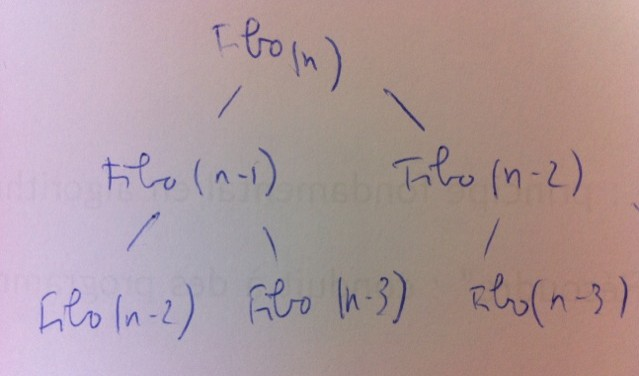
\includegraphics[width=7cm]{fibo_expo}

\paragraph{}
Réponse: on peut utiliser les techniques de marquage. Au premier passage par chaque noeud, on le marque. On évite ainsi de refaire le calcul ultérieurement.

\paragraph{}
Attention: marquer ne suffit pas, il faut également stocker le résultat. Comme la procédure Fibonnacci ne renvoie que des valeurs positives, cela peut etre fait dans le meme tableau.

Graphe des appels optimisé:\\
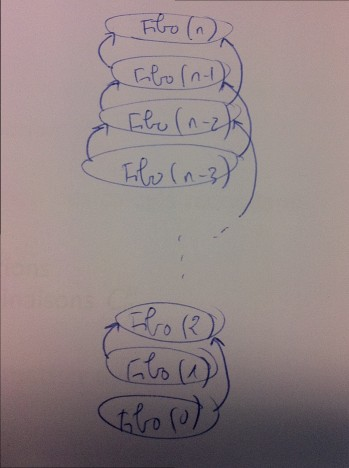
\includegraphics[width=7cm]{fibo_graph}

\paragraph{}
Version récursive avec mémorisation des nombres de fibo pour éviter la complexité exponentielle:

\begin{verbatim}
int TabFib[NMAX];
for(i=0; i < NMAX; i++)
  TabFib[i] = -1;

TabFib[0] = 0;
TabFib[1] = 1;
int Fibo(int n){
  if(TabFib[n] >= 0)
    return TabFib[n];
  else
  {
    TabFib[n] = Fibo(n-1) + Fibo(n-2);
    return TabFib[n];
  }
}
\end{verbatim}

\paragraph{}
Version itérative qui ne nécessite que 3 variables:

\begin{verbatim}
int Fibo(int n){
  int a,b,aux;
  if(n==0 || n==1)
    return n;
  else{
    a = 0;
    b = 1;
    for(i=2; i <= n; i++){
      aux = b;
      b = a+b;
      a = aux;
    }
    return b;
  }
}
\end{verbatim}

\end{exercice}

\begin{exercice}{Combinaisons $C_n^p$}

\begin{verbatim}
int Comb(int n, int p){
  if(p==0 || p==n)
    return 1;
  else
    return (Comb(n-1,p) + Comb(n-1,p-1));
}
 \end{verbatim}

\paragraph{}
Soit A(n,p) le nombre d'appels à C, y compris le principal, lors de l'évaluation de C(n,p).
En étudiant l'algorithme naif, on a:

\[
\begin{disarray}{r c l}
A(n,0) &=& A(n,n) = 1\\
0 \leq p < n : A(n,p) &=& 1 + A(n - 1, p) + A(n-1, p-1)
\end{disarray}
\]

On a donc : $A(n,p) \geq C(n,p)$\\\\

\[
 C(2k, k) = \frac{2k*(2k-1)*...*(k+1)}{k*(k-1)*...*1}
\]

\paragraph{}
Arbre des appels\\
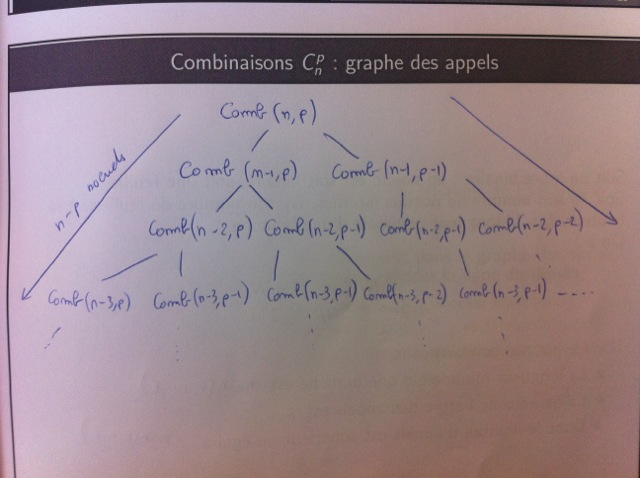
\includegraphics[width=15cm]{combinaison_appels}

\paragraph{}
Dans le cas des combinaisons:
\begin{itemize}
 \item La longueur minimale d'une branche est $min(p, n-p)$
 \item La hauteur de l'arbre des appels est $n$
 \item Donc le nombre d'appels est supérieur ou égal à $2^{min(p, n-p)}$
\end{itemize}

\paragraph{}
Matrice n x p ou tableau (n-p) x p\\
Initialisation à -1

\begin{verbatim}
 int Comb(int n, int p){
  if(p==0 || p==n)
    return 1;
  else{
    if(tab[n][p] == -1){
      tab[n][p] = Comb(n-1, p-1) + Comb(n-1,p);
    }
    return tab[n][p];
  }
}
\end{verbatim}

Cout en $O(np)$ opérations\\
Place mémoire: $(np - p^2) : O(np)$

\paragraph{Algorithme itératif}
\begin{verbatim}
 // Initialisation tab(i) = C(i,i) = 1
pour i dans 1..p faire tab(i) := 1

pour k dans 1..n-p faire
  pour i dans 1..p faire
    tab(i) := tab(i) + tab(i-1);

return tab(p);
\end{verbatim}



\end{exercice}

\section{TD6}

\paragraph{Solution récursive naïve}

\begin{verbatim}
Appel initial :

int Dist(char *A, char *B, int i, int j){
   if(j==0){
      if(i==0)
         return 0;
      else{
         return(D(A[i])+Dist(A,B,i-A,j));
      }
   }else if (i==n)
      return(T(B[j] + Dist(A,B,i,j-1))
   else
      return Min(S(A[i],B[j])+Dist(A,B,i-1,j-1),
         D(A[i]) + Dist(A,B,i-1,j),
         I(B[j])+Dist(A,B,i,j-1));
}
\end{verbatim}        	
	
\paragraph{Graphe des appels}

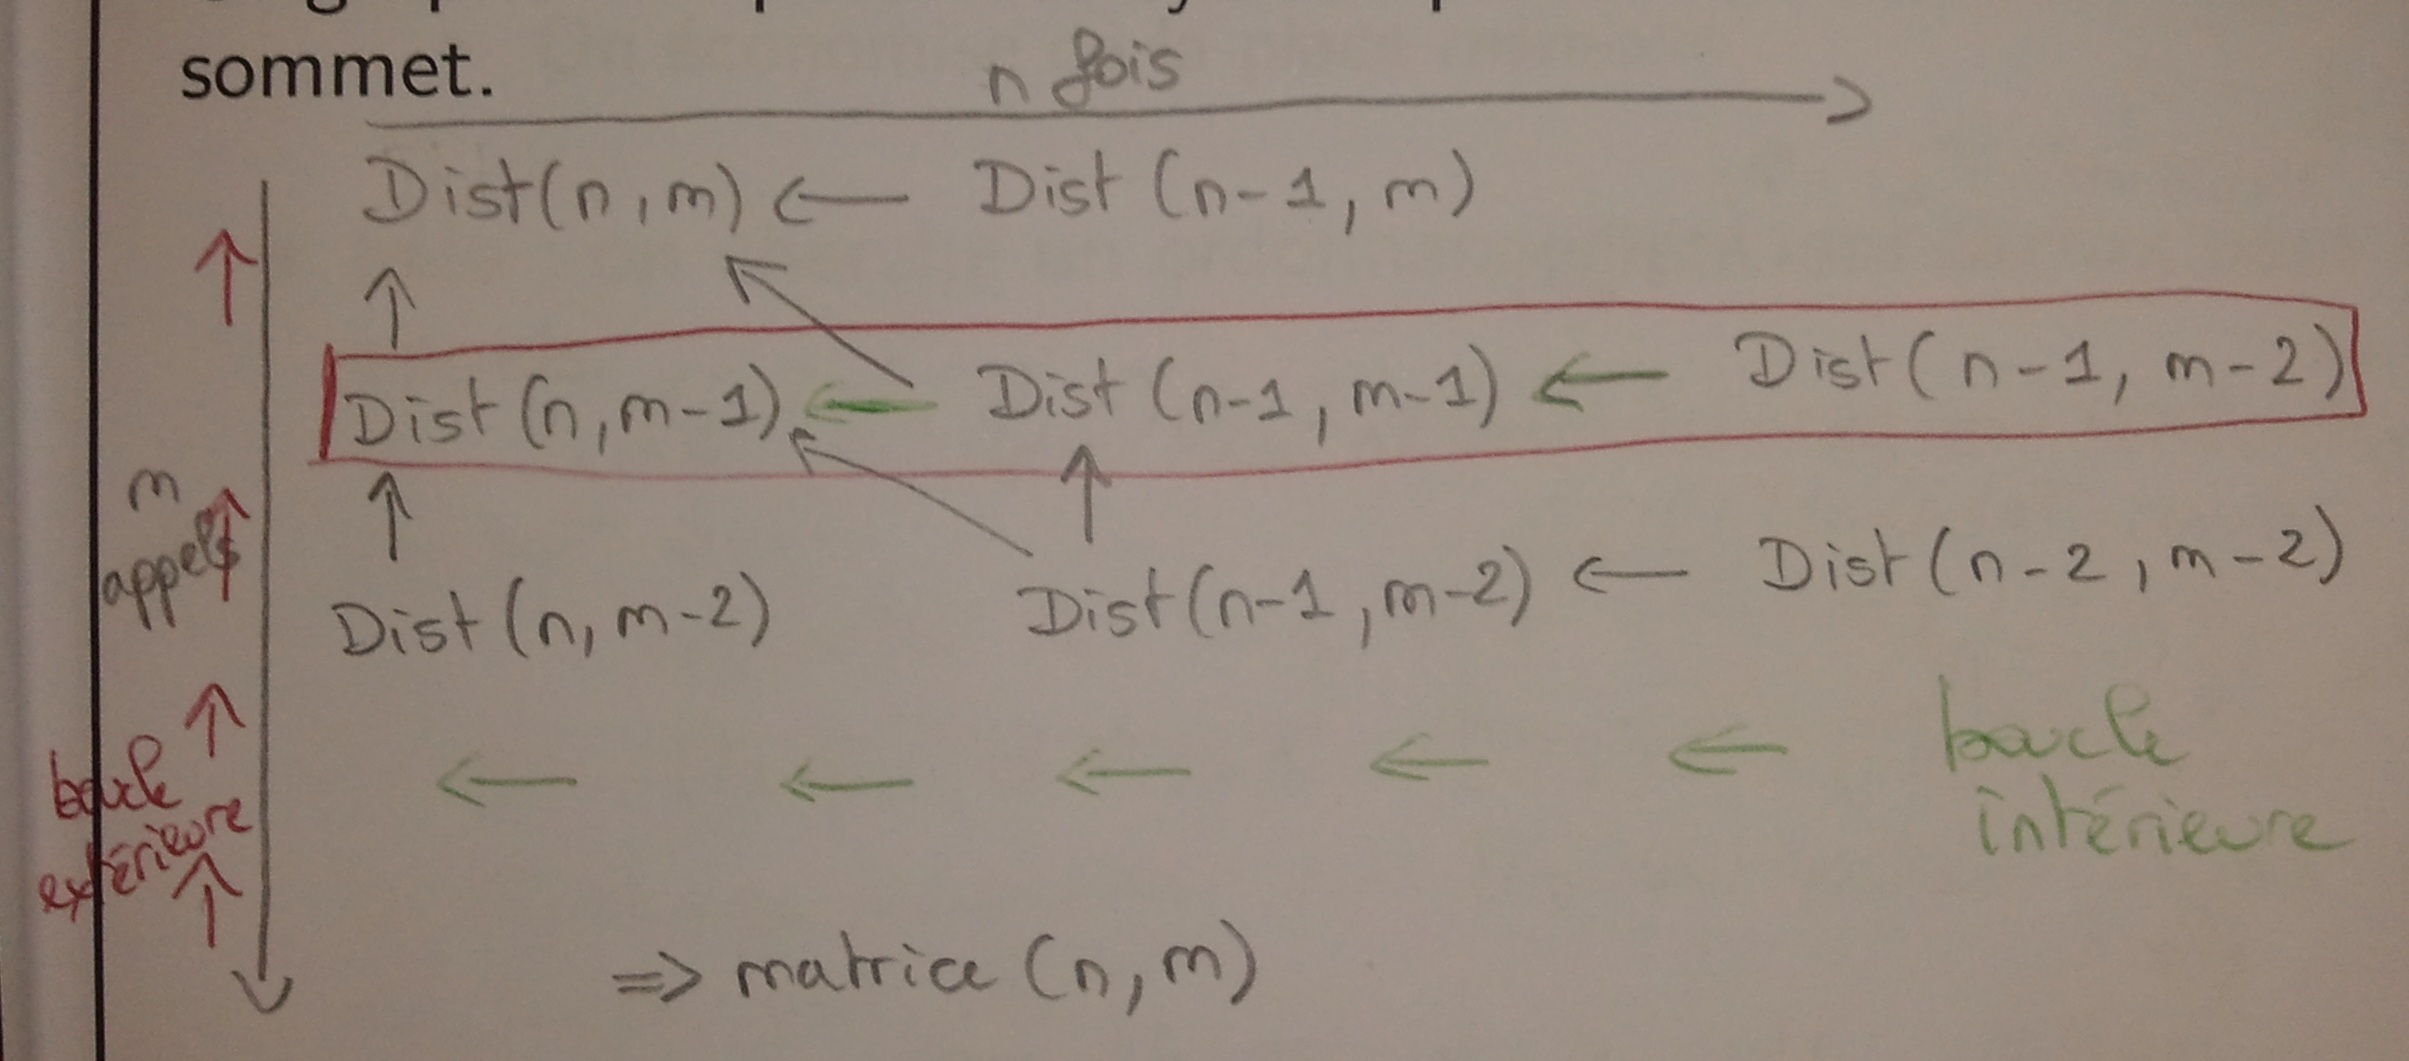
\includegraphics[width=15cm]{Photo0090}

\paragraph{Elimination des redondances}

\begin{itemize}
\item On élimine les calculs redondants à l'aide d'une technique de marquage.
\item On utilise un tableau auxilliaire TabDist de taille \textit{n} x \textit{m} (la taille est égale au nombre de sommets du graphe des appels).
\item On prend comme convention de l'initialiser à -1 pour indiquer qu'un sommet n'est pas marqué.
\end{itemize}

\paragraph{Algorithme sans les redondances}
\begin{verbatim}

int Dist(char *A, char *B, int i, int j){
   if(TabDist[i][j] != -1)
      return TabDist[i][j];
   else{
      if(j==0){
         if(i==0){
            TabDist[i][j] = 0;
            return TabDist[i][j];
         }
         else{
            TabDist[i][j] = D(A[i])+Dist(A,B,i-A,j);
            return TabDist[i][j];
         }
      }else if (i==n){
         TabDist[i][j] = T(B[j] + Dist(A,B,i,j-1)
         return TabDist[i][j];
      }else{
         TabDist[i][j] = Min(S(A[i],B[j])+Dist(A,B,i-1,j-1),
            D(A[i]) + Dist(A,B,i-1,j),
            I(B[j])+Dist(A,B,i,j-1));
         return TabDist[i][j];
      }
   }
}
\end{verbatim}
\paragraph{Calcul du coût}

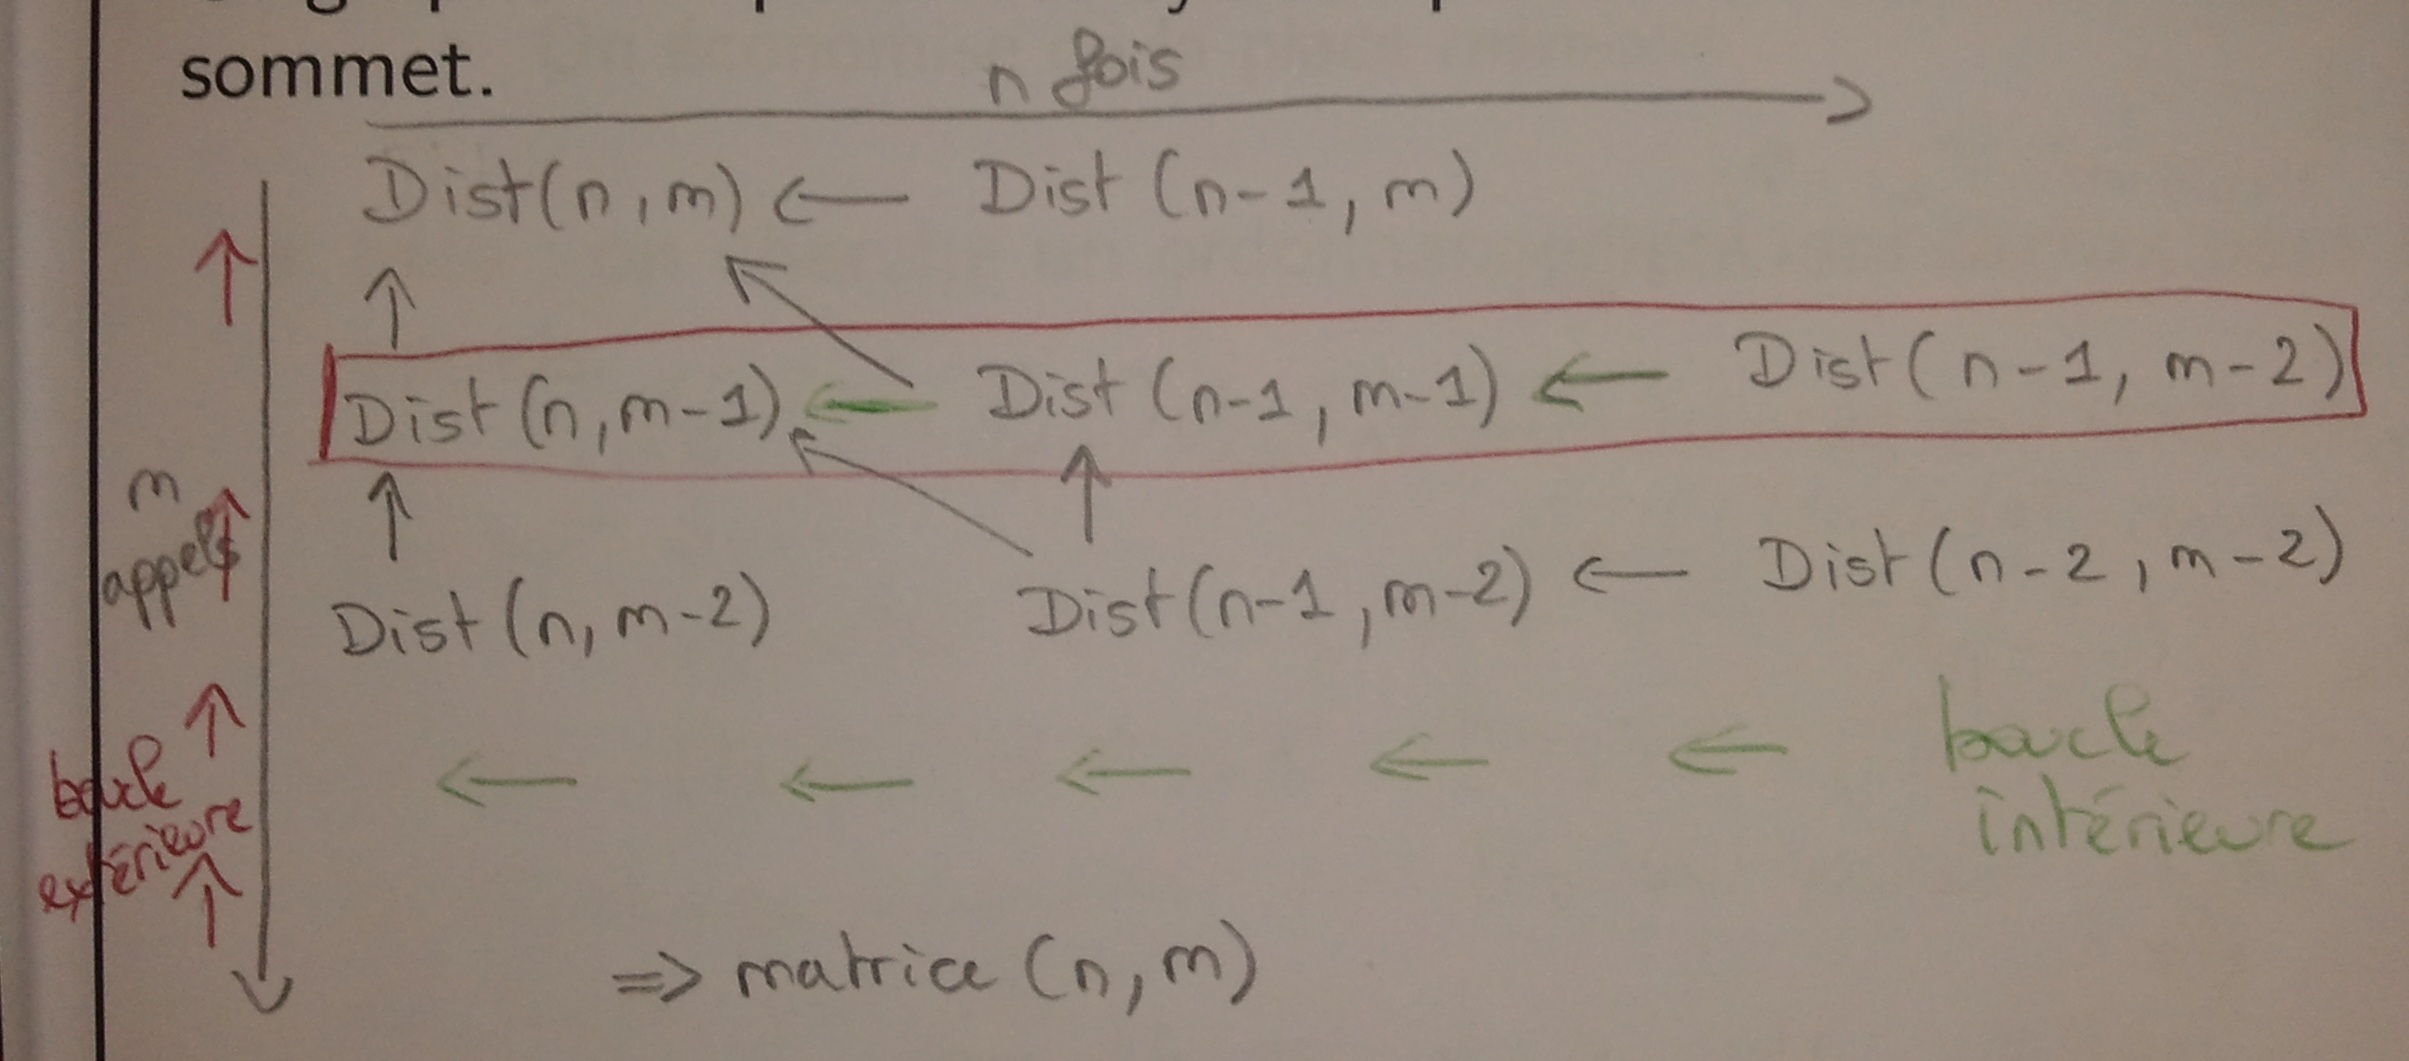
\includegraphics[width=15cm]{Photo0090}
voir les traits rouges et verts.


\paragraph{Solution itérative}
On remarque que les rôles de n et m sont symétriques. On peut donc :
\begin{itemize}
\item Remonter le long des colonnes(n=< m)
\item Remonter le long des lignes (n>m)
\end{itemize}
Le stockage mémoire est limité à min(n,m) (dernière colonne ou ligne calculée


\paragraph{Algorithme itératif}

\begin{verbatim}
On suppose (n=<m)

int Dist(char *A, char *B, int i, int j){
   int TabDist[n+1];
   int aux,tmp;
   TabDist[0]=0;
   for(i=1 ; i<=n ; i++){
      TabDist[i] = TabDist[i-1] + D(A[i]);
      //calcul de la 1ère colonne
   }
   for(j=1 ; j<=m ; j++){
      aux = TabDist[0];
      for(i=1 ; i<=n ; i++){
         tmp = TabDist[i];
         TabDist[i][j] = Min(S(A[i],B[j])+aux,
            D(A[i]) + TabDist[i-1],
            I(B[j])+tmp);
         aux = tmp;
      }
   }
   return TabDist[n];
}
\end{verbatim}

\paragraph{Reconnaissance de chaines de caractères bruités : exemple}

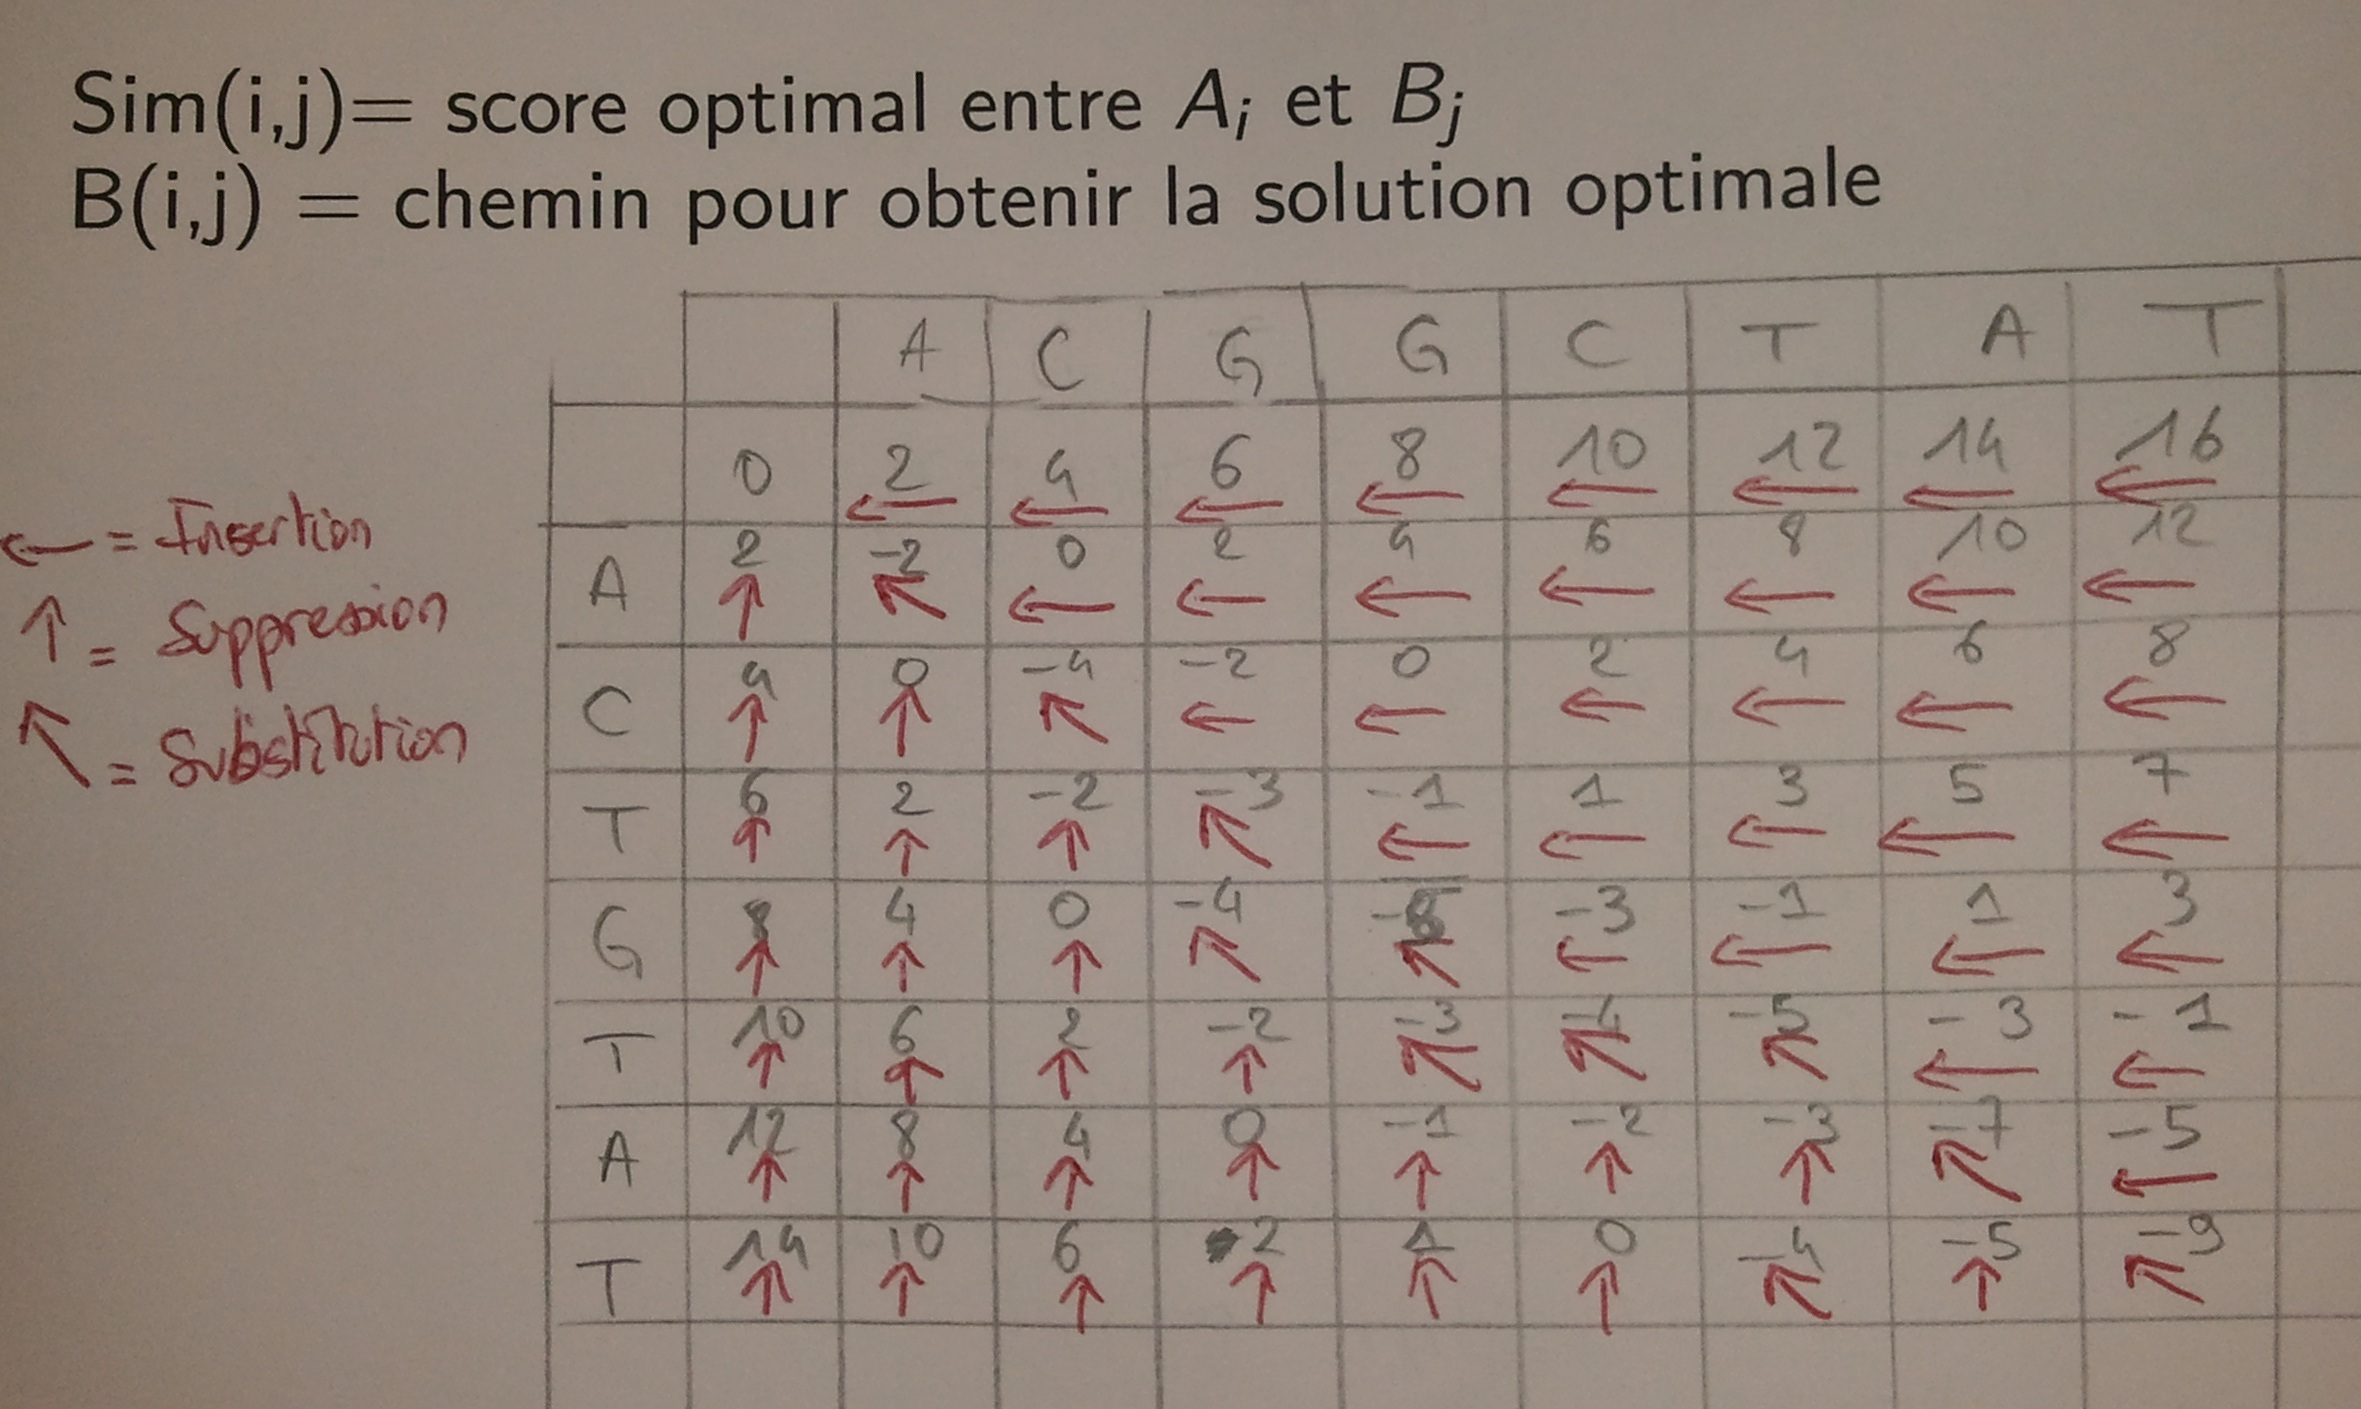
\includegraphics[width=15cm]{Photo0089}

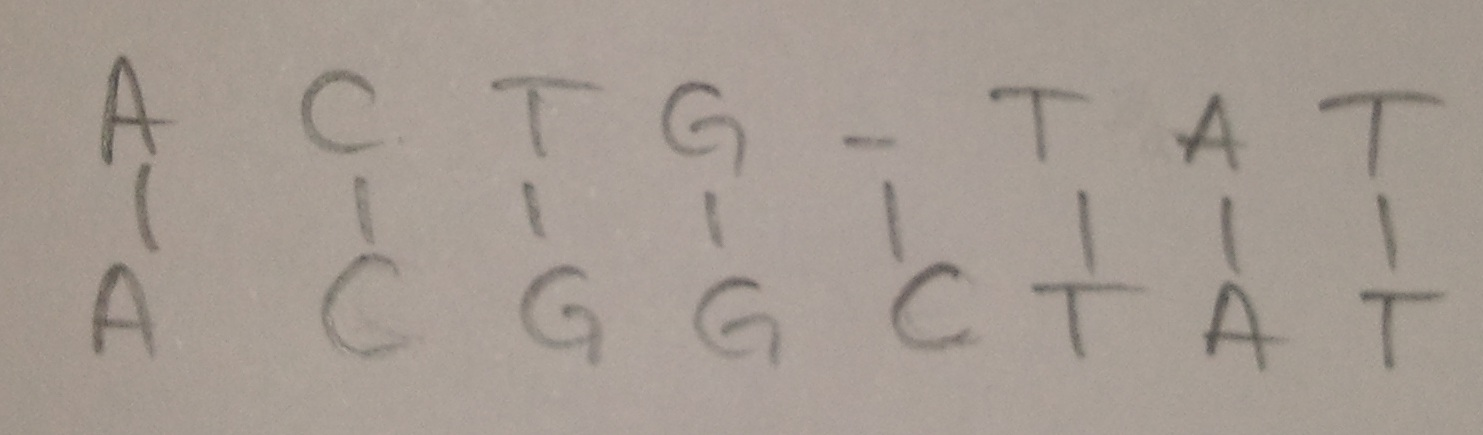
\includegraphics[width=15cm]{Photo0091}

On prend le chemin depuis (n,m) en utilisant S.

\paragraph{Un premier exemple}

1) ((M1 M2) M3) M4\\
   100x1x50 + 100x50x20 + 100x20x1 = 17 000\\
   
2) (M1 (M2 M3)) M4\\
   5 000\\
   
3) (M1 M2)(M3 M4)\\
   11 000\\

4) M1 (M2 (M3 M4))\\
   1150\\

5) M1 ((M2 M3) M4)\\
   1120\\
   
Cout minimum : 5) avec 1120
 
\paragraph{Solution récursive naïve}

\begin{verbatim}
Appel initial : Mult(1,n).

int Mult(int i, int j){
   int min, tmp;
   if(i==j)
      return 0;
   else{
      min = Mult(i,j) + Mult(i+1,j + d[i] d[i+1] d[j+1];
      for(k=i+1 ; k<j ; k++){
         tmp = Mult(i,k)+Mult(k+1,j) + d[i] d[k+1] d[j+1];
         if(tmp<min) min = tmp;
      }
      return min;
   }
}
\end{verbatim}
\paragraph{Calcul du cout de la solution naïve}
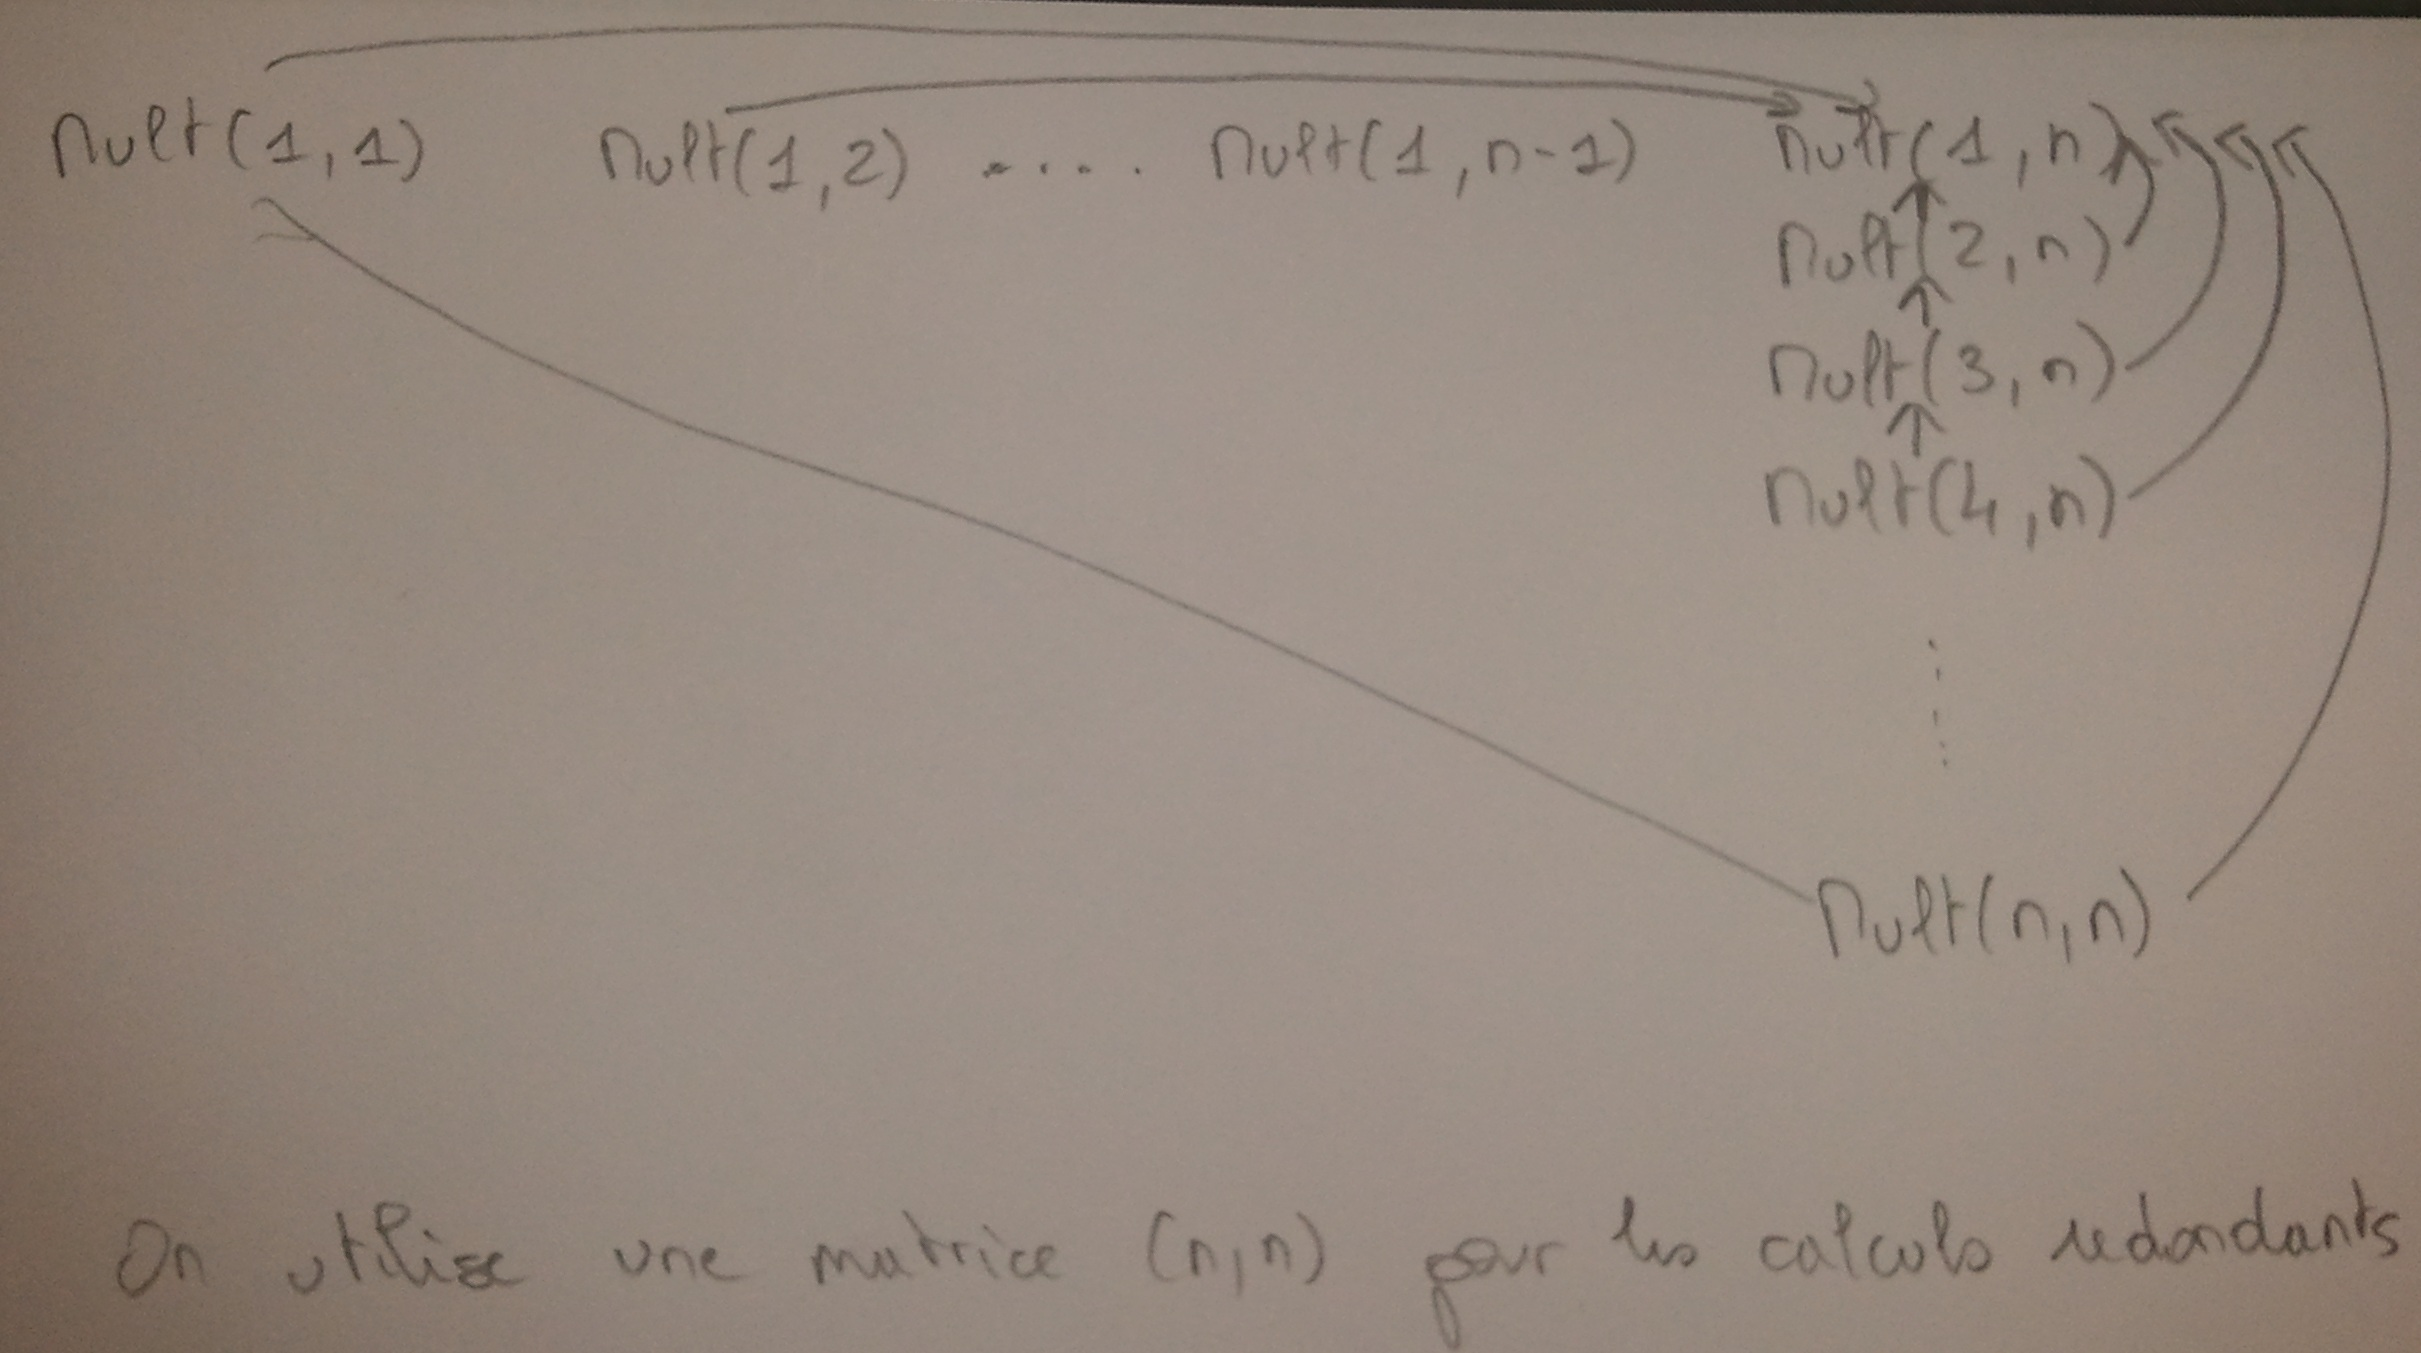
\includegraphics[width=15cm]{Photo0092}
On utilise une matrice (n,n) pour les calculs redondants.

\paragraph{Elimination des calculs redondants}
\begin{verbatim}
Appel initial : Mult(1,n).

int Mult(int i, int j){
   int min, tmp;
   if(TabMult[i][j] == -1)
      if(i==j){
         TabMult[i][j]=0
         return 0;
      }
      else{
         min = Mult(i,j) + Mult(i+1,j + d[i] d[i+1] d[j+1];
         for(k=i+1 ; k<j ; k++){
            tmp = Mult(i,k)+Mult(k+1,j) + d[i] d[k+1] d[j+1];
            if(tmp<min) min = tmp;
         }
         TabMult[i][j] = min;
   }
   return TabMult[i][j];
}
\end{verbatim}

\end{document}